Up to this point, we have investigated the numeric capabilities of Mathcad.  In this section, we learn about the calculus and symbolic capabilities of Mathcad.  


\section{Mathcad: Calculus}\label{sec:Mathcad_calculus}

\noindent \large \textsf{\textbf{Using the calculus toolbar }} \normalsize\\

First, open both the calculus and the the symbolic toolbar with File $>$ Toolbars $>$ Calculus, and File $>$ Toolbars $>$ Symbolic.

\index{Mathcad!Toolbars!Symbolic}
\index{Mathcad!Toolbars!Calculus}
\begin{center}
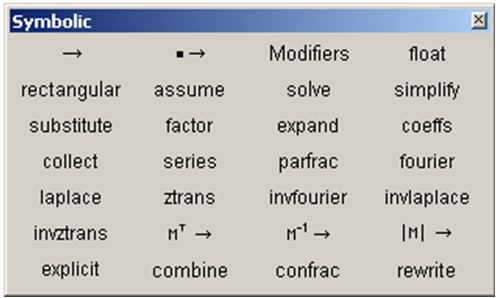
\includegraphics{figures/mathcad_symbolic_toolbar2.png}
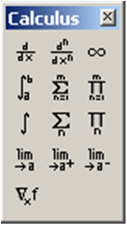
\includegraphics{figures/mathcad_calculus_toolbar.png}
\end{center}

Many of the key concepts from a two-semester sequence of Calculus courses can be found on the calculus toolbar: limits, derivatives (including the gradient), integrals (definite and indefinite), summations and products.  The symbol for infinity is also on this toolbar.
The symbolic toolbar may look a bit more complicated (it is). We will cover many of the symbolic toolbar buttons in the next section, but in order to complete many of the symbolic calculations using the calculus toolbar, we will need the ``Symbolic Evaluation'' (the $\longrightarrow$ button) from the symbolic toolbar too.  Of course, there is a shortcut for symbolic evaluation: Ctrl + . (hold the Ctrl key and press the period).

We start with some simple examples.\\

\index{Mathcad!Symbolic Evaluation}
\example{ex_calculus_01}{{\bf Compute the derivative and integral of $x^2$.}\\

By hand, we know the answers are $2x$ and $x^3/3 + C$.
Using Mathcad, we use the symbolic differentiation 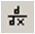
\includegraphics{figures/mathcad_symbolic_derivative_button.png} and indefinite integral 

\includegraphics{figures/mathcad_symbolic_integral_button.png} buttons.  In each case, we end the calculation with the symbolic evaulation button $\rightarrow$.\\
%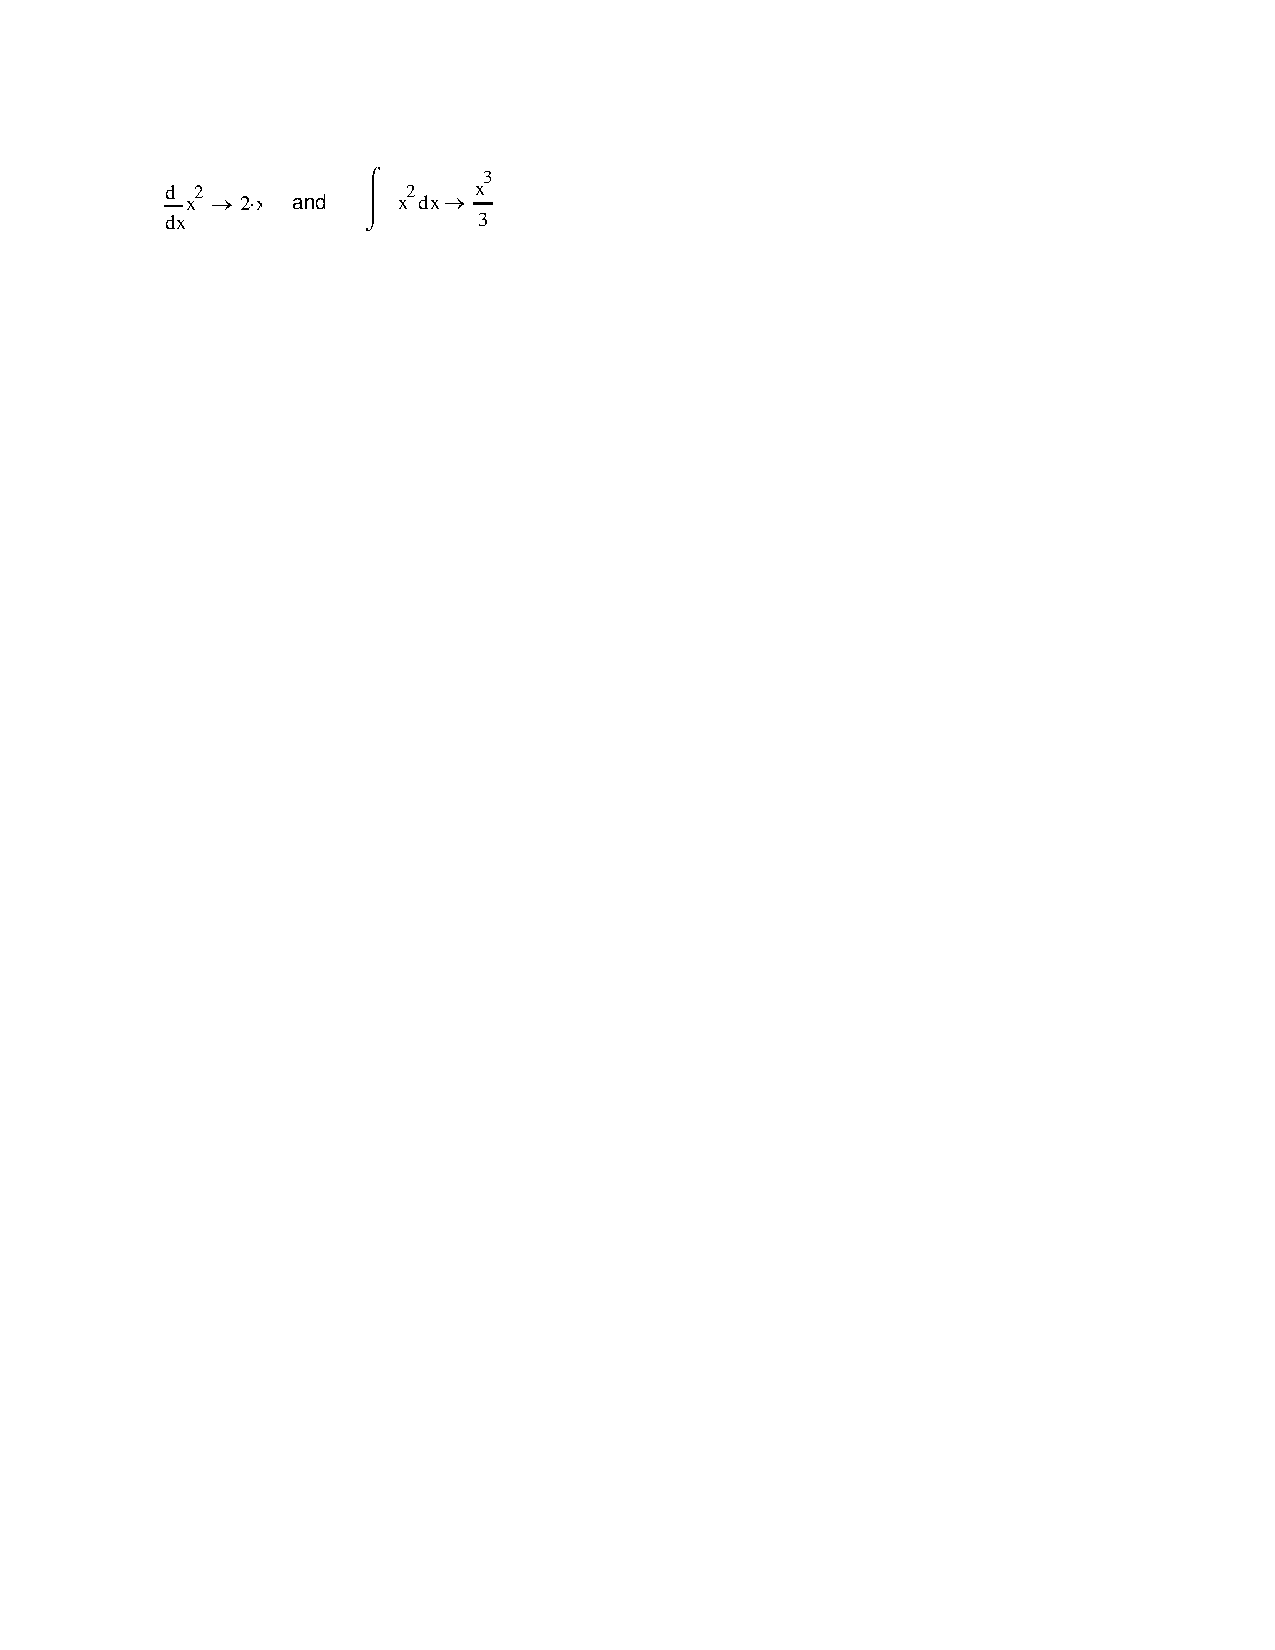
\includegraphics[bb=1in 9in 3in 10in]{figures/mathcad_symbolic_calculus1.pdf} %Mathcad copied to Word, saved as pdf, guess bounding box size
\begin{center}
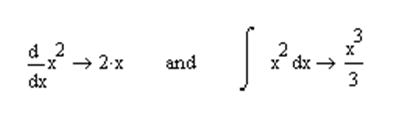
\includegraphics{figures/mathcad_symbolic_calculus_example1.png}\\
\end{center}

Note that the $+ c$ part of the indefinite integral is not shown.
}

\section{Mathcad: Symbolics}\label{sec:Mathcad_symbolics}

Here we look at many of the other capabilities of the symbolic toolbar.  The ``solve'' button was discussed in a previous chapter.\\

\index{Mathcad Functions!\tnr{expand}}
\index{Mathcad Functions!\tnr{factor}}
\index{Mathcad Functions!\tnr{series}}
\index{Mathcad Functions!\tnr{parfrac}}
\index{Mathcad Functions!\tnr{laplace}}

\example{ex_symbolic_01}{{\bf Expand $(x+2)^4$, factor $x^3 + 3x^2 + 3x +1$, find the Taylor polynomial of order 8 for $\cos x$, find the partial fraction expansion of $\displaystyle \frac{1}{x^3 - x}$, and find the Laplace transform of $t^2-1$.}\\

In each case, we enter the expression, select the button from the symbolic toolbar, make any alterations (like in the Taylor polynomial question - adding the comma and 8) and click outside the expression
\begin{center}
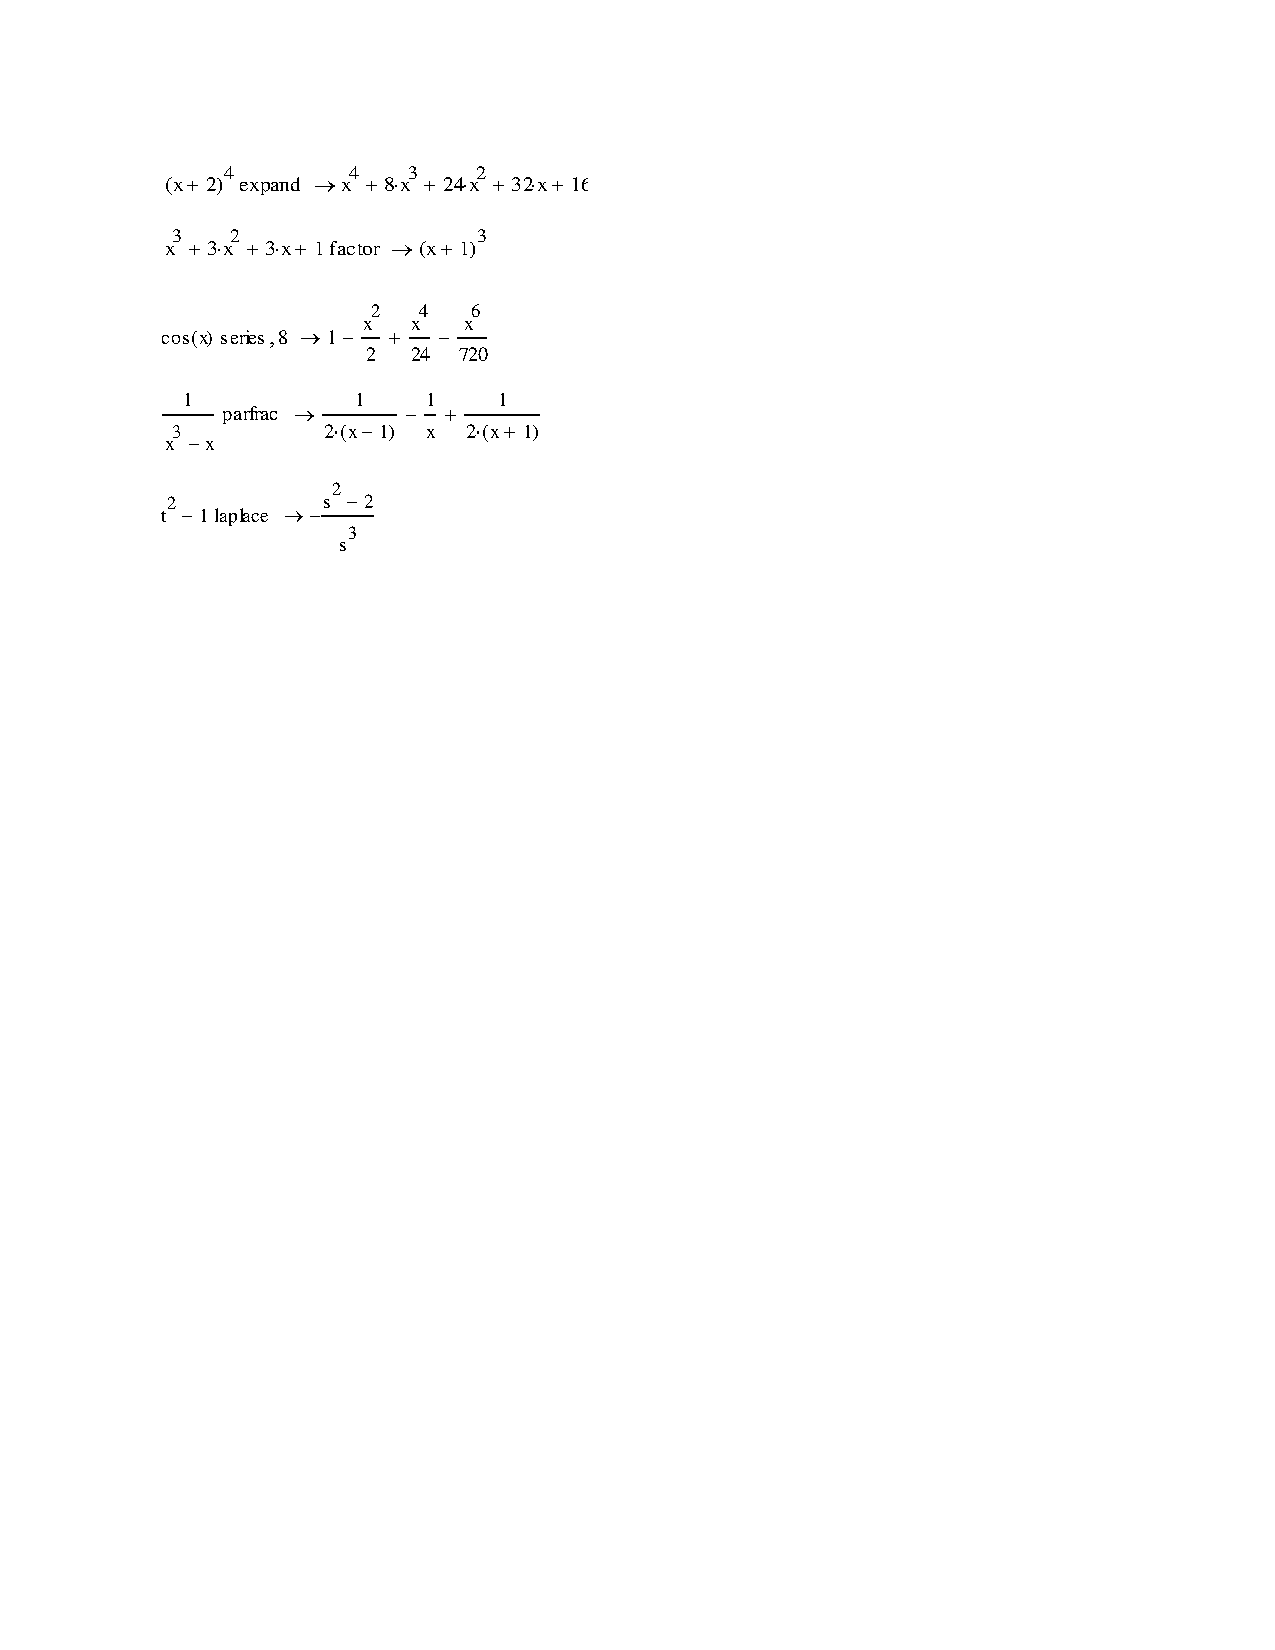
\includegraphics[bb=1in 7.5in 3in 10in]{figures/mathcad_symbolic1.pdf} %Mathcad copied to Word, saved as pdf, guess bounding box size
\end{center}
}
\\
In the next example, we point out the difference between symbolic evaluation and approximation.\\

\example{ex_calculus_02}{{\bf The Error Function}\\

The error function $f(t)$ comes up in many applications.  It is defined as\\
\begin{center}
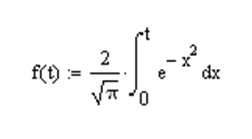
\includegraphics{figures/mathcad_calculus_erf1.png}\\
\end{center}

If we use the standard symbolic evaluation symbol $\longrightarrow$, then we will get the answer in terms of the built in error function ``erf''
\begin{center}
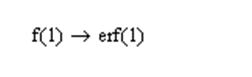
\includegraphics{figures/mathcad_calculus_erf2.png}\\
\end{center}

If we instead use the evaluation equals sign (just $=$), we get the approximation
\begin{center}
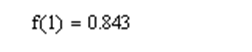
\includegraphics{figures/mathcad_calculus_erf3.png}\\
\end{center}
}

\newpage
\printexercises{exercises/17_exercises}
